\section{Отслеживание контакта и моделирование трения}

Для наглядности мы ограничиваемся рассмотрением омни-колес, 
оснащенных четырьмя роликами. Также для простоты сами ролики имеют оси 
вращения, лежащие в плоскости колеса (Рис.~\ref{OmniWheel}).

\begin{figure}[htb]
\centering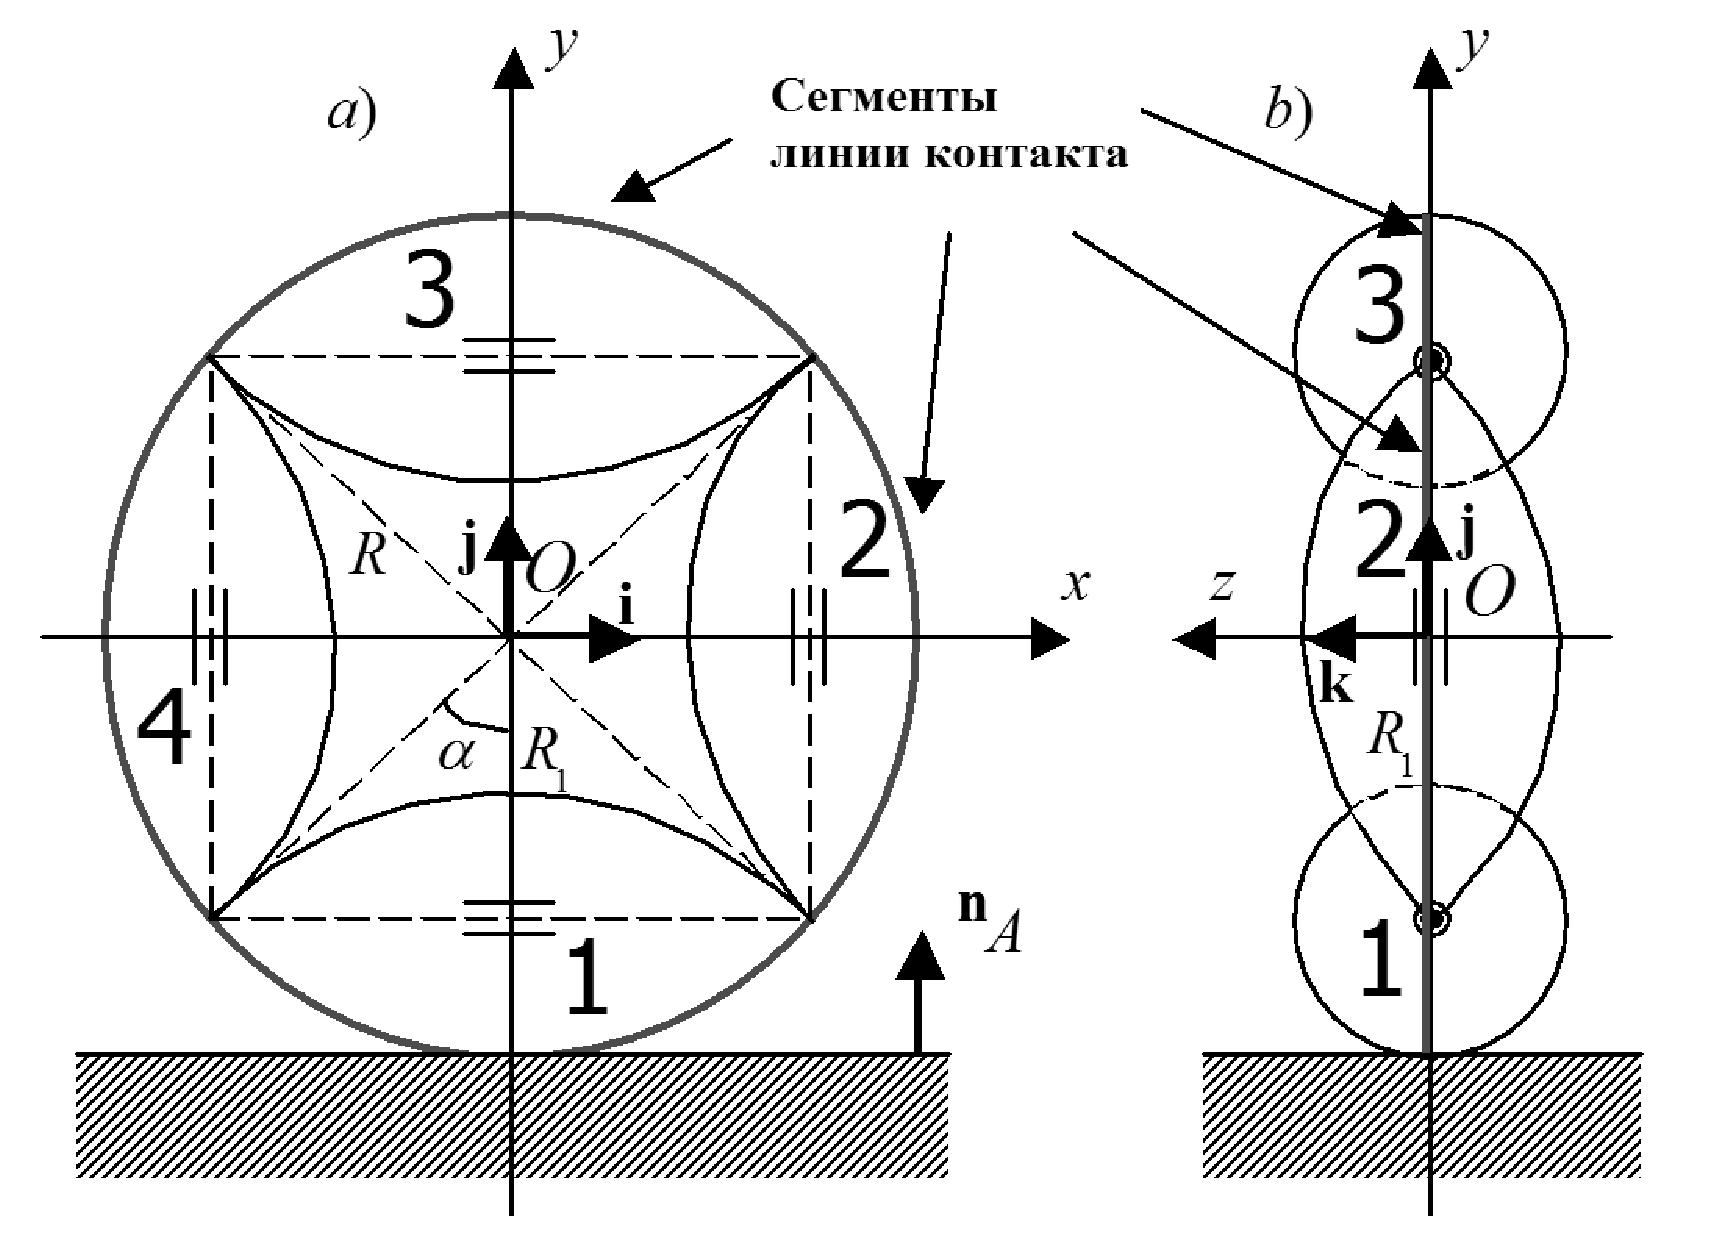
\includegraphics[width=13cm]{content/parts/3_friction/nd/OmniWheel.eps}
\caption{Омни-колесо в вертикальном положении: a) вид сбоку; b) вид спереди.}
\label{OmniWheel}
\end{figure}

Предполагается также, что ролики размещаются на колесе таким образом, что для 
вертикально поставленного омни-колеса проекция линии контактирования наинизшего 
ролика с горизонтальной плоскостью будет состоять из последовательности 
сегментов соответствующих линий контактирования отдельных роликов. Эти сегменты 
сопрягаются таким образом, что при переходе контакта от ролика к ролику 
нормальная составляющая скорости точки ролика, находящейся в точке контакта, к 
горизонтальной плоскости равна нулю. Это означает отсутствие удара по нормали к 
плоскости. В случае коллинеарности осей роликов и плоскости колеса скачки 
скорости скольжения по касательному направлению к горизонтальной плоскости 
также отсутствуют, так как при переходе контакта между роликами их внешние 
поверхности непрерывно вырождаются в точку (в идеализированной модели), что 
означает отсутствие кинематического влияния собственного вращения роликов при 
переходе контакта с ролика на ролик. Так что в результате переключение 
контактов между роликами омни-колеса не приведет к нарушению регулярности 
движения в силу причин ударного характера. Заметим еще раз, что все описанное 
будет справедливо, если колесо все время остается в вертикальном положении.

% На следующем уровне сборки модели несколько колес соединяются с подвижной 
% платформой экипажа при помощи шарнирных связей. В нашем случае количество колес 
% может быть три или более (в зависимости от конструкции экипажа и модели 
% контактирования ролика с полом). На платформе они могут образовывать самые 
% разные конфигурации. В конкретном примере Рис.~\ref{Vehicle} имеется три 
% колеса, образующие равносторонний треугольник в горизонтальной плоскости $zx$. 
% Ось $y$ здесь предполагается вертикальной.

% \begin{figure}[htb]
% \centering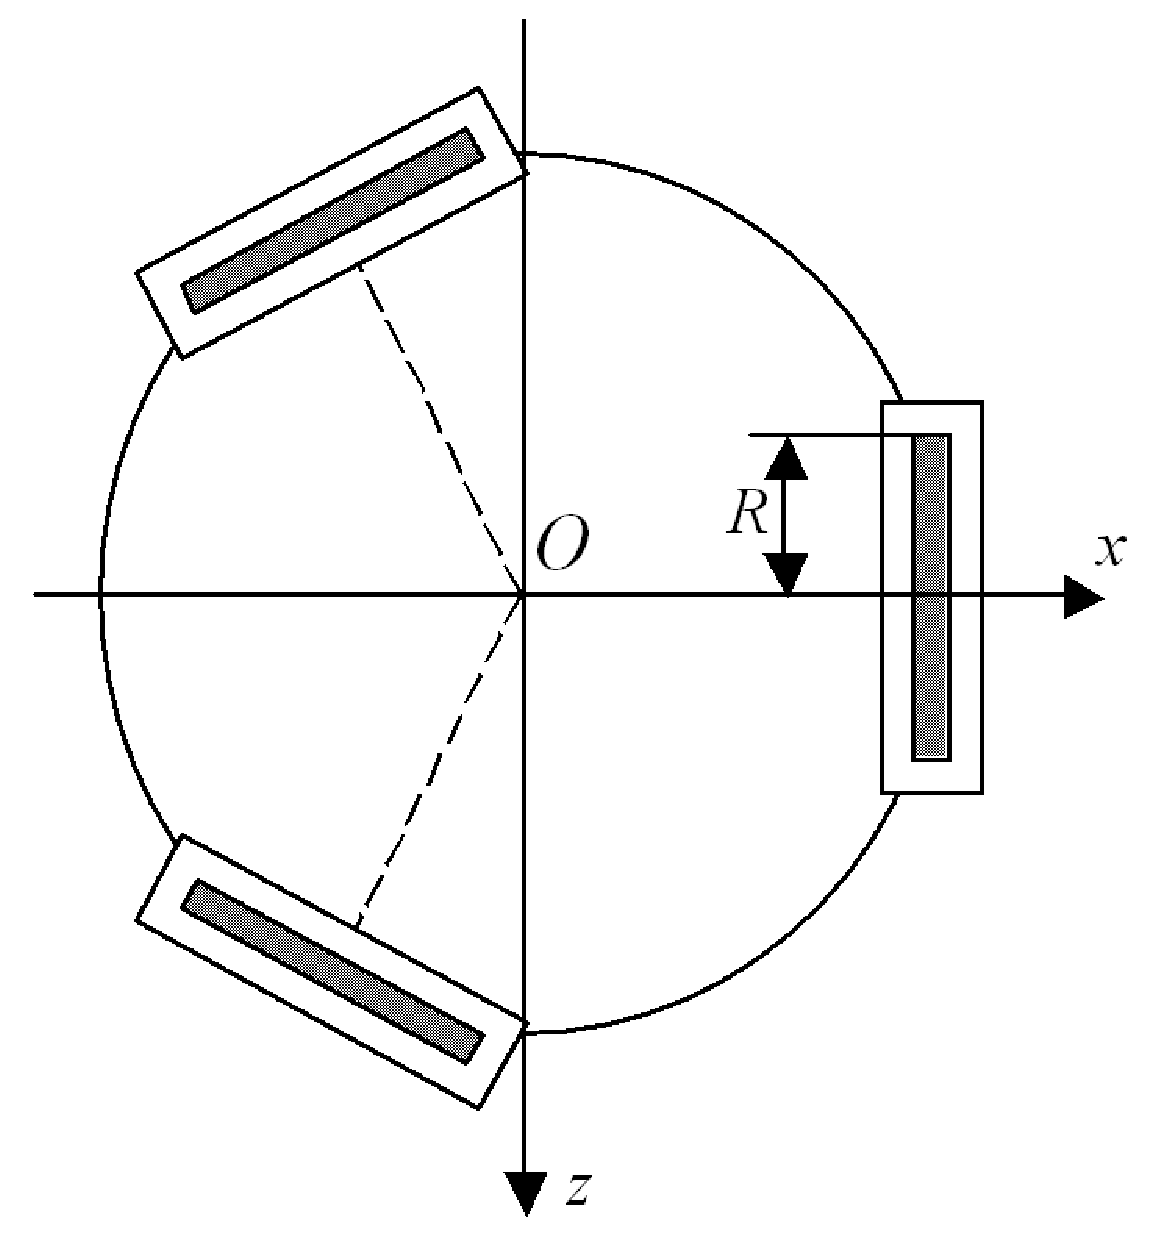
\includegraphics[width=9cm]{content/parts/3_friction/nd/Vehicle.eps}
% \caption{Трехколесный экипаж. Вид сверху.}
% \label{Vehicle}
% \end{figure}

% \section{Модель динамики отдельного ролика.\ }
\label{sec3}
Вначале предположим, что ролик представляет собой осесимметричное 
веретенообразное твердое тело с внешней поверхностью, задаваемой в своих 
собственных осях $Oxyz$ уравнением
\begin{equation}
x^2+\left(\sqrt{y^2+z^2}+R_1\right) ^2=R^2,
\label{3_1}
\end{equation}
где $R$ --- радиус омни-колеса, $R_1=R\cos{\alpha }$ --- расстояние от центра
ролика до центра колеса, $\alpha =\pi /n$ --- половина центрального угла, под
которым ролик виден из центра колеса, $n$ --- количество роликов на колесе.

\begin{figure}[htb]
\centering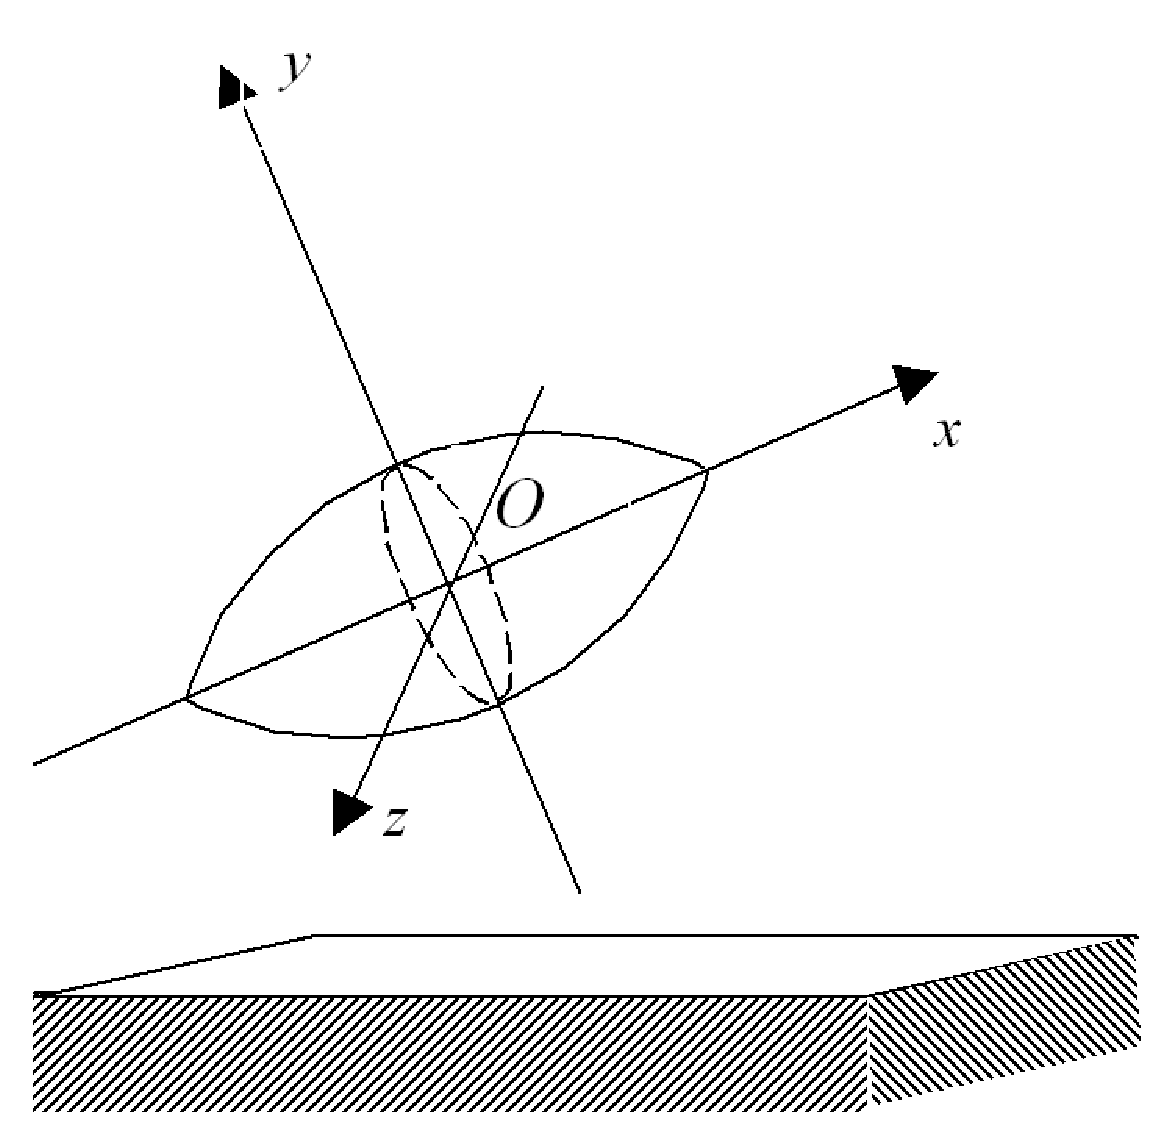
\includegraphics[width=10cm]{content/parts/3_friction/nd/Roller.eps}
\caption{Ролик над горизонтальной плоскостью. Вид сбоку.}
\label{Roller}
\end{figure}

Динамика поступательно-вращательного движения реализуется так, как это описано
в~\cite{Kosenko2007}, в виде уравнений Ньютона -- Эйлера. Причем для 
моделирования вращательного движения твердого тела используется алгебра 
кватернионов~\cite{KosenkoQuaternionRus,Kosenko1998}.

Отдельную проблему представляет задача отслеживания контакта между поверхностью 
ролика и горизонтальной плоскостью. Для моделирования динамики твердого тела с
неудерживающей связью применена технология, описанная в~\cite{Kosenko2006}. В
данном случае можно было бы применить систему алгебраических или 
дифференциально-алгебраических уравнений. Однако эти уравнения вырождаются в 
точках $x=\pm R\sin\alpha $ в координатах ролика. Такое вырождение обычно 
приводит к аварийному завершению вычислительного процесса моделирования.

В нашей задаче положение спасает специфика конфигурации, обеспечивающей 
постоянство вертикального расположения омни-колес. При этом условии можно
указать явную формулу, позволяющую вычислить ближайшую к плоскости точку $P_B$
ролика (Рис.~\ref{ContactScheme}). Этой точке всегда <<противостоит>> её 
вертикальная проекция $P_A$ на плоскость (Рис.~\ref{ContactScheme}).

\begin{figure}[htb]
\centering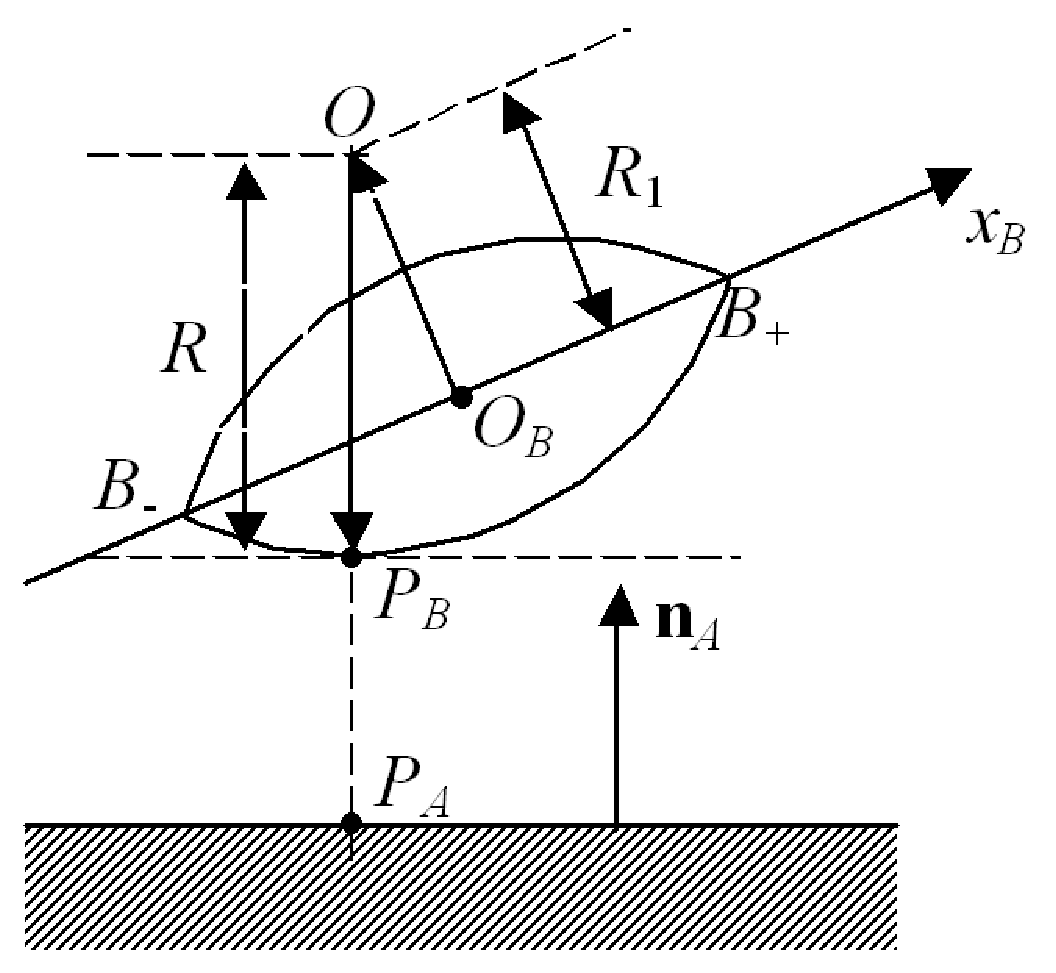
\includegraphics[width=8cm]{content/parts/3_friction/nd/RollerSection.eps}
\caption{Схема отслеживания контакта: вид сбоку отдельного ролика.}
\label{ContactScheme}
\end{figure}

Обозначим символом ${\bf i}_B=(1,0,0)^T$ орт собственной оси ролика $O_Bx_B$.
Этот вектор представлен в системе координат ролика $O_Bx_By_Bz_B$. Пусть $T_B$
--- матрица поворота ролика относительно инерциальной системы координат 
$O_Ax_Ay_Az_A$, связанной с неподвижной плоскостью. Пусть также ${\bf r}_B$ ---
радиус-вектор геометрического центра ролика в текущий момент времени и 
${\bf n}_A=(0,1,0)^T$ --- орт нормали (восходящей вертикали) к плоскости. 
Плоскость условно обозначается нами телом с индексом $A$, ролик --- $B$. Пусть
${\bf d}$ --- горизонтальный орт, вычисляемый по формуле
$$
{\bf d}=\dfrac{T_B{\bf i}_B\times {\bf n}_A}
              {\left| T_B{\bf i}_B\times {\bf n}_A\right|}.
$$
Тогда, очевидно, отрезок $\overrightarrow{O_BO}$, расположенный в вертикальной
плоскости, будет иметь длину $R_1$ и задаваться формулой
$$
\overrightarrow{O_BO}=R_1{\bf d}\times T_B{\bf i}_B.
$$
Здесь $O$ --- центр кривизны окружности вертикального сечения ролика 
(Рис.~\ref{ContactScheme}). Так что самая нижняя точка $P_B$ внешней 
поверхности ролика будет задаваться по формуле
\begin{equation}
{\bf r}_{P_B}={\bf r}_B+R_1{\bf d}\times T_B{\bf i}_B-R{\bf n}_A,
\label{3_2_0}
\end{equation}
поскольку точка $P_B$ лежит на упоминавшейся выше окружности на общей вертикали 
с точкой $O$. Для вычисления положения точки $P_A$ нужно вторую координату 
вектора ${\bf r}_{P_B}$ положить равной нулю
\begin{equation}
{\bf r}_{P_A}=\left( x_{P_B},0,z_{P_B}\right) ^T.
\label{3_2_1}
\end{equation}

Вся описанная выше вычислительная процедура будет справедлива только, если 
вектор $T_B{\bf i}_B$ имеет направление, ограниченное по вертикали углами
$\pm\alpha $. Если соответствующий угол превышает значение $\alpha $, то 
следует положить $P_B=B_{-}$, где $B_{-}$ --- левая концевая точка ролика. Если
же этот угол меньше величины $-\alpha $, нужно положить $P_B=B_{+}$, где 
$B_{+}$ --- правая концевая точка ролика.

В конечном итоге условие контактирования ролика и плоскости можно записать в 
виде
\begin{equation}
\left| T_B{\bf i}_B\cdot {\bf n}_A\right|\le\sin\alpha .
\label{3_2}
\end{equation}
Это условие, однако, позволяет из всего множества роликов колеса выделить 
нижний (контактирующий) и верхний. Чтобы отбросить случай последнего ролика
можно к последнему условию присоединить также требование 
\begin{equation}
y_B<R,
\label{3_3}
\end{equation}
где $y_B$ --- высота центра ролика относительно инерциальной системы координат.

Таким образом, конъюнкция условий (\ref{3_2}) и (\ref{3_3}) означает наличие
контакта. В противном случае, при отсутствии контакта, нормальная реакция 
отсутствует (закон Синьорини). С другой стороны, реализация контакта 
геометрически означает выполнение скалярного условия 
\begin{equation}
y_{P_B}=0,
\label{3_4}
\end{equation}
а его отсутствие --- также скалярного (альтернативного) условия
$$
F_n=0,
$$
где $F_n$ --- нормальная составляющая реакции (в данном случае отсутствующей) 
приложенной в точке $P_B$.

% \begin{figure}[htb]
% \centerline{
% 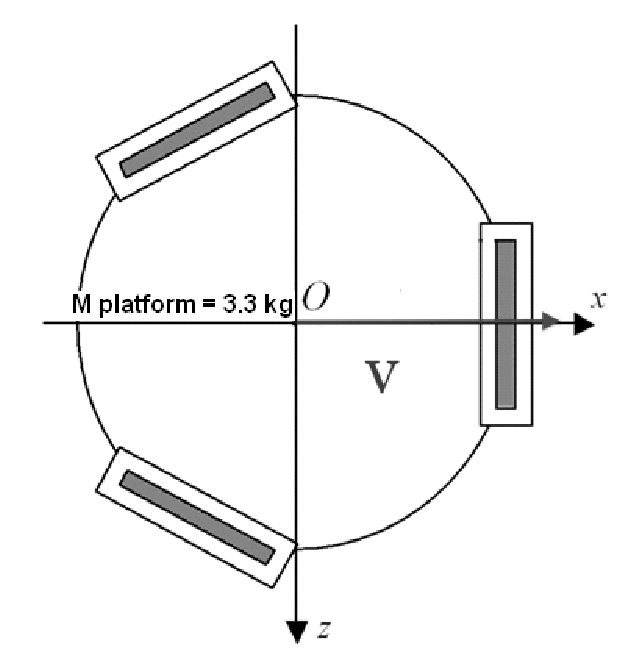
\includegraphics[width=7cm]{content/parts/3_friction/nd/Translat.eps}
% 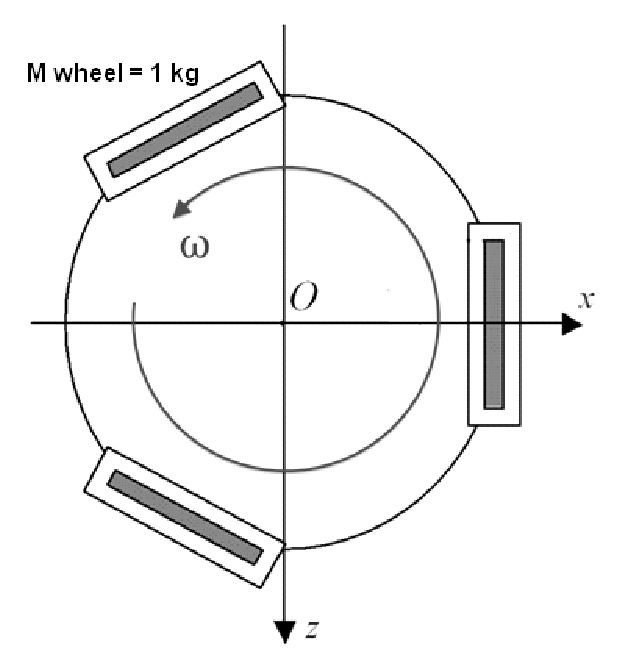
\includegraphics[width=7cm]{content/parts/3_friction/nd/Rotat.eps}
% }
% \caption{Типы движения при верификации модели.}
% \label{TypesOfMotion}
% \end{figure}

Вычислительная практика показала, что уравнения контакта в форме (\ref{3_4})
стабильно приводит к аварийному завершению процесса симуляции динамической 
модели ролика. Аналогичный результат получается, если в качестве уравнения 
контактирования использовать уравнение вида 
$$
v_n=0,
$$
где $v_n$ -- нормальная составляющая скорости точки контактирования, лежащей
на теле $B$, относительно тела $A$ (горизонтальной плоскости). И только 
уравнение вида
$$
\dot{v}_n=0
$$
приводит к требуемому результату -- корректной работе объекта контактирования
(реализованного в данном случае на языке Modelica~\cite{Fritzson}) в процессе 
симуляции модели. Вся реализация процесса контактирования 
выполнена в предположении точечного <<твердого>> контакта твердых тел без 
какой-либо податливости.

Колеса, собранные в экипаж, с неизбежностью будут сохранять вертикальное 
положение. Поэтому упрощенный алгоритм отслеживания контакта, описанный выше,
всегда будет работать правильно.
